\documentclass[11pt,a4paper]{scrartcl}
\usepackage{graphicx}
\usepackage[ngerman]{babel}
\usepackage[utf8]{inputenc}
\usepackage[colorlinks=false,pdfborder={0 0 0}]{hyperref}
\usepackage{longtable}
\usepackage{listings}
\lstset{breaklines=true, breakatwhitespace=true, basicstyle=\small}

\title{Netzwerksicherheit Labor 1\\
	Testen von Firmen-Netzwerken}
\author{Yanick Eberle\\
		Pascal Schwarz}
\date{}
\begin{document}
\maketitle
\tableofcontents
\newpage
\section{Aufgabe 1 - Wireshark/ARP}
\subsection{Protokollaufbau}
Die folgende Grafik\footnote{Quelle: http://ipv6.com/images/diagrams/arp1.gif} zeigt den Aufbau des Protokolls.
\begin{figure}[h]
	\centering
	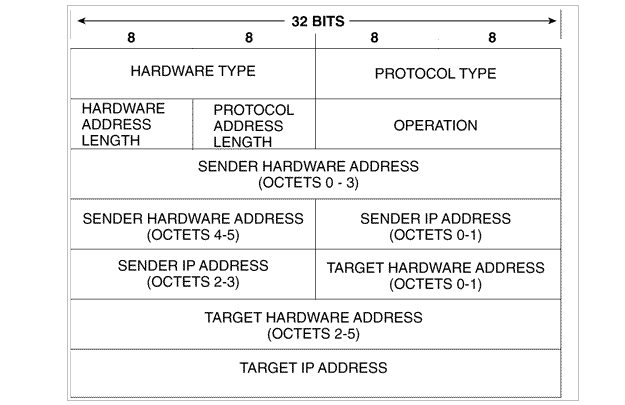
\includegraphics[width=0.7\textwidth]{../aufg1/arp1.png}
	\caption{Address Resolution Protocol}
	\label{fig:arp}
\end{figure}
\subsection{Beantwortung der gestellten Fragen zum Protokoll}
\textbf{Wieviele Bytes ist das ARP Opcode-Feld vom Anfang des Ethernet Frames entfernt?} \\6 Byte\\
\textbf{Welcher Wert hat das Opcode-Feld innerhalb des ARP-payload des Ethernet frame, worin eine ARP Anfrage gestellt ist?} \\ARP request\\
\textbf{Enthält die ARP Meldung die IP Adresse des Senders?} \\Ja\\
\textbf{Wo in der ARP-Anfrage erscheint die "Frage" : Welche Maschine besitzt diese IP Adresse?} \\Operation (Opcode)\\
\textbf{Geben Sie den Inhalt des ARP-Cache Ihres Laptops an, und erklären Sie, was jede
Spalte bedeutet.} \\arp -n\\

\begin{tabular}{l|l|l|l|l|l}
	Address & HWtype & HWaddress & Flags & Mask & Iface \\
	10.196.134.1	&	ether	&	ee:ee:ee:01:07:06	&	C	&	&	eth0 \\
	10.196.134.127	&	ether   &	54:42:49:56:7c:bc	&	C	&	&	eth0
\end{tabular}
\begin{description}
	\item[Address] zu welcher IP gehört der Rest der Information in der Zeile?
	\item[HWType] gibt layer1/2 typ an
	\item[HWAddress] der IP (Spalte 1) zugeordnete Hardwareadresse (hier MAC-Adresse)
	\item[Flags] C steht für Complete (ARP Anfrage abgeschlossen), M wäre permanent, P publish
	\item[Mask] würde zusammen mit publish benutzt
	\item[Iface] über welches Interface ist die HWAddr erreichbar
\end{description}


\newpage
\section{Aufgabe 2 - Utilities ping, hping3, dig, traceroute}
\subsection{Perl Script für Host-Discovery im Subnet}
\lstinputlisting[numbers=left]{../aufg2/netscan.pl}

Das Script erzeugt eine Ausgabe ähnlich der Folgenden:
\begin{lstlisting}
10.196.134.1
10.196.134.16
10.196.134.17
10.196.134.19
10.196.134.21
10.196.134.118
10.196.134.120
\end{lstlisting}

\subsection{DNS Protokoll}
Viele Informationen in diesem Abschitt stammen von \url{http://doc-tcpip.org/Dns/named.dns.message.html}.
\subsubsection{DNS-Request Packet: Welches Protokoll wird benutzt? Welche Vorteile bietet
dies für einen DNS?}
Es wird UDP als Transportprotokoll (siehe Grafik \ref{fig:dns_2_2_1} auf Seite \pageref{fig:dns_2_2_1}) eingesetzt. Dadurch entsteht weniger Overhead (hauptsächlich weil kein 3-way-Handshake nötig ist), was wiederum die Performance erhöht (geringere Latenz).
\begin{figure}[h]
	\centering
	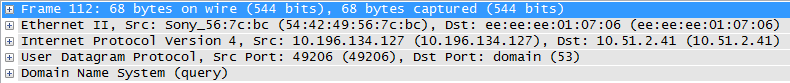
\includegraphics[width=1.0\textwidth]{../aufg2/dns_2_2_1.png}
	\caption{DNS Anfrage in Wireshark}
	\label{fig:dns_2_2_1}
\end{figure}

\subsubsection{DNS-Request Paket: Welcher src und dst port werden definiert? Wie interpretieren Sie das Resultat?}
Auf Zielhost wird auf Port 53 abgehört. Da es eine Anfrage ist, ist der Destination Port 53. Siehe hierzu Grafik \ref{fig:dns_2_2_2} auf Seite \pageref{fig:dns_2_2_2}.
\begin{figure}[h]
	\centering
	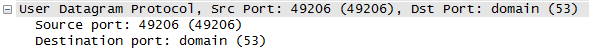
\includegraphics[width=1.0\textwidth]{../aufg2/dns_2_2_2.png}
	\caption{DNS Ports in Wireshark}
	\label{fig:dns_2_2_2}
\end{figure}

\subsubsection{DNS-Response Paket: Welche Felder gibt es? Erklären Sie deren Bedeutung.}
\begin{description}
	\item[Time] Antwortzeit
	\item[Transaction ID] eindeutige Nummer, muss mit Transaction ID des DNS Requests übereinstimmen, ist dies nicht der Fall, muss die Antwort verworfen werden.
	\item[Flags] Request, Response, Error, no Error, \ldots
	\item[Questions] Anzahl Anfragen
	\item[Answer RRs] Anzahl Antworten
	\item[Authority RRs] RRs, die auf verantwortliche Server deuten
	\item[Additional RRs] RRs mit weiteren Informationen/Records
\end{description}
\textbf{RR} steht hier für \textbf{Resource Record}, ein Format zur Angabe des Mappings von IP-Adresse zu Name bzw. umgekehrt - oder weitere Information. Resource Records sind die Einträge in den Datenbank-Files des Name Servers.
\begin{figure}[h]
	\centering
	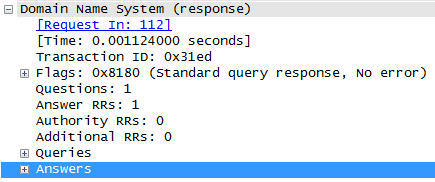
\includegraphics[width=0.7\textwidth]{../aufg2/dns_2_2_3.png}
	\caption{Header in DNS Response}
	\label{fig:dns_2_2_3}
\end{figure}

\subsubsection{DNS-Response Paket: Was enthält das Feld Answer? Erklären Sie jede zusätzliche
Information, die Sie in diesem Feld gefunden haben.}
\begin{description}
	\item[NAME] Der Domain-Name, zu der dieser RR gehört. 
	\item[TYPE] Der RR-Typ Code. Spezifiziert die Bedeutung des Feldes RDATA. Zwei Oktets. 
	\item[CLASS] RR-Klasse. Spezifiziert die Bedeutung des Feldes RDATA. Zwei Oktets. 
	\item[TTL] Time To Live - eine 32-bittige Zahl, die die Anzahl der Sekunden angibt, für die man diesen Record im Cache behalten darf. Null bedeutet, das dieser RR nur für die aktuelle Transaktion gilt. 
	\item[RDLENGTH] Eine 16-bittige Zahl, die die Anzahl der Oktets im RDATA Feld angibt. 
	\item[RDATA] Ein String variabler Länge (Oktets), der die Resource beschreibt. Das Format hängt von den Setzungen in TYPE und CLASS ab. Bei TYPE = A und CLASS = IN wäre das also eine normale 4 Oktet (32-bittige) ARPA Internet Adresse.
\end{description}
\begin{figure}[h]
	\centering
	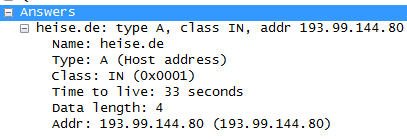
\includegraphics[width=0.7\textwidth]{../aufg2/dns_2_2_4.png}
	\caption{Answer-Abschnitt einer Response}
	\label{fig:dns_2_2_4}
\end{figure}

\subsection{Traceroute apple.com}
Die geographische Lage der Router kann insbesondere in diesem Beispiel über die reverse DNS Einträge festgelegt werden. So ist beispielsweise *.zrh1.he.net in Zürich. Der Sprung passiert folglich zwischen Hop 13 und 14, also zwischen Amsterdam und Washington.

Grundsätzlich sollte der Sprung an der Latenzzeit ersichtlich sein. In diesem Fall ist die Latenzzeit der Router in Frankfurt und Amsterdam jedoch schon sehr hoch, was ev. auf eine Überlastung am Übergang zwischen he.net und xo.net in Frankfurt (am DE-CIX) zurückzuführen ist.
\begin{figure}[h]
	\centering
	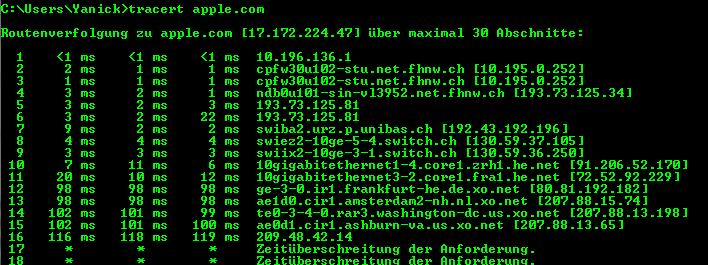
\includegraphics[width=1.0\textwidth]{../aufg2/tracert_apple.png}
	\caption{Traceroute zu apple.com}
	\label{fig:traceroute_apple}
\end{figure}

\newpage
\section{Aufgabe 3 - Nmap/Wireshark}
Wir haben den Aufruf folgendermassen gemacht: \begin{verbatim}nmap -P0 -p80 www.fhnw.ch\end{verbatim} Wir haben die Option -P0 gesetzt, weil wir wissen, dass unter www.fhnw.ch (mindestens) ein Server erreichbar ist. Der Output des Commands war der folgende:

\begin{lstlisting}
Starting Nmap 6.01 ( http://nmap.org ) at 2012-11-15 08:18 CET
Nmap scan report for www.fhnw.ch (147.86.3.160)
Host is up (0.0021s latency).
rDNS record for 147.86.3.160: wsnmu25.fhnw.ch
PORT   STATE SERVICE
80/tcp open  http
Nmap done: 1 IP address (1 host up) scanned in 0.03 seconds
\end{lstlisting}

Mit dem Output können wir praktisch den gesamten aufgezeichneten Verkehr (siehe Grafik \ref{fig:traffic_nmap-p80} auf Seite \pageref{fig:traffic_nmap-p80} begründen:
\begin{itemize}
	\item Der Name muss zu einer IP (hier 147.86.3.160) aufgelöst werden, was mittels DNS geschieht.
	\item Die IP wird zurück zu einem Namen aufgelöst (reverse DNS Lookup, "rDNS record..."), ebenfalls via DNS.
	\item Danach wird ein kompletter TCP-3-way-Handshake durchgeführt und die Verbindung danach sofort wieder beendet (Frame 8 mit TCP Flags RST,ACK).
	\item Da der TCP-Handshake erfolgreich durchgeführt werden konnte zeigt uns nmap an, dass der Port geöffnet ist.
\end{itemize}

\begin{figure}[h]
	\centering
	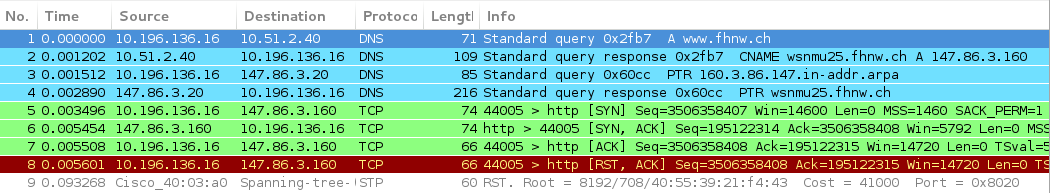
\includegraphics[width=1.0\textwidth]{../aufg3/traffic_nmap-p80.png}
	\caption{Datenverkehr, der durch den nmap-Aufruf ausgelöst wurde}
	\label{fig:traffic_nmap-p80}
\end{figure}

\newpage
\section{Aufgabe 4 - Installation Metasploit}
Metaplsploit wurde unter Arch Linux mithilfe des Pakets von \url{https://aur.archlinux.org/packages.php?ID=2880} installiert. Das Package beinhaltet Postgresql nicht, daher musste dieser Datenbankdienst separat über die Paketverwaltung installiert und danach konfiguriert werden. Die Administration von Postgresql wurde mit dem Paket pgadmin abgewickelt (Erstellen eines Benutzers und einer Datenbank).
Nach diesen Schritten wurde metasploit folgendermassen fertig eingerichtet:
\begin{lstlisting}
$ sudo msfupdate
$ gem install pg
$ msfconsole
msf > db_connect metasploit:****@127.0.0.1/metasploit
\end{lstlisting}
Nach diesen Schritten ist metasploit bereit für Scans und mit der Datenbank verbunden.


\newpage
\section{Aufgabe 5 - Footprinting/Scanning}
\subsection{Footprinting}
\subsubsection{Whois fhnw.ch}
\begin{lstlisting}
Domain name:
fhnw.ch

Holder of domain name:
Fachhochschule Nordwestschweiz FHNW
Graf Heinz
ICT Kommunikation
Steinackerstrasse 5
CH-5210 Windisch
Switzerland
Contractual Language: German

Technical contact:
Fachhochschule Nordwestschweiz FHNW
Graf Heinz
ICT Kommunikation
Steinackerstrasse 5
CH-5210 Windisch
Switzerland

DNSSEC:N

Name servers:
ns.inwx.de
ns1.fhnw.ch [147.86.3.20]
ns2.fhnw.ch [147.86.3.21]
\end{lstlisting}

\subsubsection{DNS Einträge}
\begin{figure}[p]
	\centering
	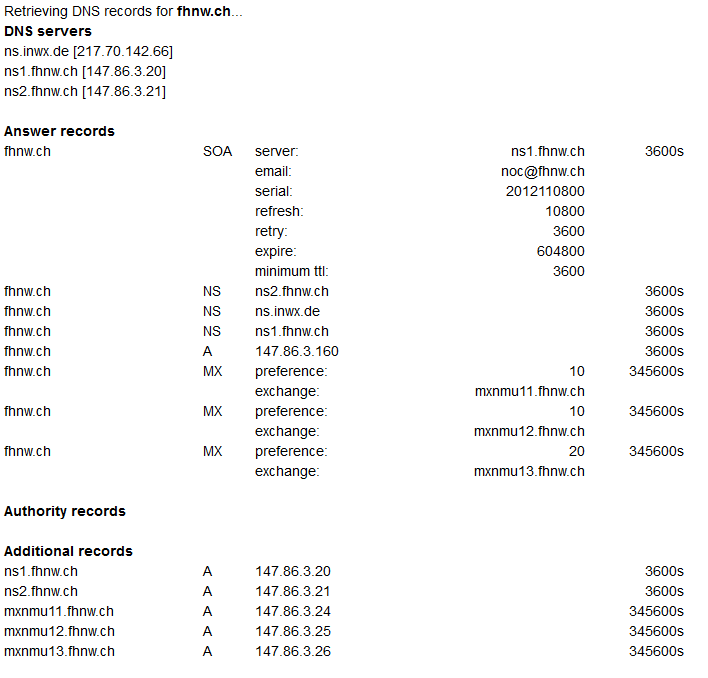
\includegraphics[width=0.6\textwidth]{../aufg5/dns_records.png}
	\caption{DNS Einträge fhnw.ch}
	\label{fig:dns_records}
\end{figure}

\subsubsection{Infos zur Website}
Die Informationen in Grafik \ref{fig:website_infos} auf Seite \pageref{fig:website_infos} stammen von \url{http://www.websitelibrary.ch/fhnw.ch}.
\begin{figure}[p]
	\centering
	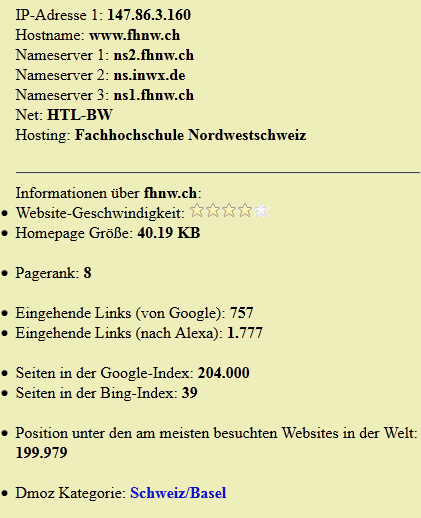
\includegraphics[width=0.5\textwidth]{../aufg5/website_infos.png}
	\caption{Informationen zu www.fhnw.ch}
	\label{fig:website_infos}
\end{figure}

\subsubsection{Informationen zu Mail und Netzwerk}
Eberle: Quellenangabe hier bitte - Grafik \ref{fig:iprange_infos} auf Seite \pageref{fig:iprange_infos}
\begin{figure}[p]
	\centering
	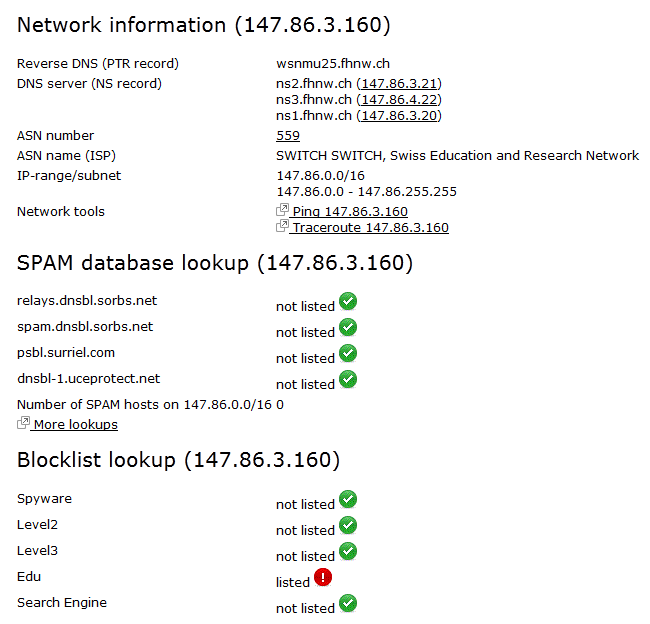
\includegraphics[width=0.6\textwidth]{../aufg5/iprange_infos.png}
	\caption{Informationen zu Mail und Netzwerk}
	\label{fig:iprange_infos}
\end{figure}

\subsubsection{Informationen zum Leiter Netzwerkteam}
Die Grafik \ref{fig:heinz_graf1} auf Seite \pageref{fig:heinz_graf1} zeigt die Informationen über Heinz Graf auf der FHNW-Website.

Gemäss \url{http://www.bienen-ag.ch/index.php?option=com_content&view=article&id=193} ist er auch Beisitzer im Verband Aargauischer Bienenzüchtervereine.
\begin{figure}[p]
	\centering
	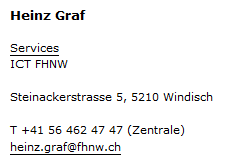
\includegraphics[width=0.4\textwidth]{../aufg5/heinz_graf1.png}
	\caption{Informationen zu Heinz Graf von der FHNW Website}
	\label{fig:heinz_graf1}
\end{figure}

\subsubsection{Via Google gefundene Informationen}
Die Anfrage \textbf{site:fhnw.ch} sowie weitere Anfragen in der Form \textbf{site:fhnw.ch -site:www.fhnw.ch} lieferte u.A. die folgenden Treffer:
\begin{lstlisting}
www.fhnw.ch
www0.fhnw.ch
web.fhnw.ch
webtransfer.fhnw.ch
weblogin.fhnw.ch
webmail.fhnw.ch
sapportal.fhnw.ch
pms.fhnw.ch
www.students.fhnw.ch
webcorp2.fhnw.ch
blogs.fhnw.ch
eranger.fhnw.ch
es.fhnw.ch
aai-logon.fhnw.ch
helio.i4ds.technik.fhnw.ch
tools.fhnw.ch
www.ph.fhnw.ch
portfolio-kompetenzmanagement.fhnw.ch
mediothek.hgk.fhnw.ch
status.fhnw.ch
ict.campus-brugg-windisch.fhnw.ch
pensentool.fhnw.ch
genius.wirtschaft.fhnw.ch
m.fhnw.ch
*.imvs.technik.fhnw.ch (diverse Subdomains)
*.cs.technik.fhnw.ch (diverse Subdomains)
\end{lstlisting}
Mit \textbf{link:fhnw.ch} konnten u.A. folgende Einträge gefunden werden:
\begin{lstlisting}
www.unilu.ch/deu/links_4006.html
lib.consortium.ch/html_wrapper.php?dir=libraries&src=addresses1
www.kgv.ch/links
www.swissdigin.ch/apps/swissdigin.nsf/de/leitfaeden
www.i4ds.ch/team.html
www.esski.ch/
www.ftal.net/UEber-uns.73.0.html
www.esbasel.ch/en/impressum/
\end{lstlisting}

\subsubsection{Reverse-DNS-Namen von 147.86.0.0/16}
Für die Reverse-DNS-Namen wurde folgendes Perl Skript verwendet:
\lstinputlisting[numbers=left]{../aufg5/nslookup.pl}

In der folgenden Tabelle sind die PTR-Einträge im DNS für die externe IP-Range der FHNW gelistet.
\begin{longtable}{p{2.5cm}|p{7cm}}
	\textbf{IP Adresse} & \textbf{PTR-Eintrag} \\
	\endfirsthead
	\textbf{IP Adresse} & \textbf{PTR-Eintrag} \\
	\endhead
	\multicolumn{2}{l}{\textit{Fortführung auf nächster Seite\ldots}} \\
	\endfoot
	\endlastfoot
	147.86.3.160 & wsnmu25.fhnw.ch \\
	147.86.3.161 & wsnmu25-sec1.fhnw.ch \\
	147.86.3.162 & wsnmu25-sec2.fhnw.ch \\
	147.86.3.163 & wsnmu25-sec3.fhnw.ch \\
	147.86.3.164 & wsnmu32.fhnw.ch \\
	147.86.3.165 & wsnmu32-sec1.fhnw.ch \\
	147.86.3.166 & wsnmu32-sec2.fhnw.ch \\
	147.86.3.167 & wsnmu32-sec3.fhnw.ch \\
	147.86.3.168 & wsnmu32-sec4.fhnw.ch \\
	147.86.3.169 & wsnmu32-sec5.fhnw.ch \\
	147.86.3.170 & wsnmu31.fhnw.ch \\
	147.86.3.171 & wsnmu31-sec1.fhnw.ch \\
	147.86.3.172 & wsnmu31-sec2.fhnw.ch \\
	147.86.3.173 & wsnmu31-sec3.fhnw.ch \\
	147.86.3.174 & wsnmu31-sec4.fhnw.ch \\
	147.86.3.175 & wsnmu31-sec5.fhnw.ch \\
	147.86.3.176 & wsnmu33.fhnw.ch \\
	147.86.3.177 & wsnmu33-sec1.fhnw.ch \\
	147.86.3.178 & wsnmu33-sec2.fhnw.ch \\
	147.86.3.179 & wsnmu33-sec3.fhnw.ch \\
	147.86.3.180 & wsnmu33-sec4.fhnw.ch \\
	147.86.3.182 & wsnmu14.fhnw.ch \\
	147.86.3.183 & wsnmu37.fhnw.ch \\
	147.86.3.184 & wsnmu37-sec1.fhnw.ch \\
	147.86.3.185 & wsnmu37-sec2.fhnw.ch \\
	147.86.3.186 & wsnmu37-sec3.fhnw.ch \\
	147.86.3.187 & wsnmu37-sec4.fhnw.ch \\
	147.86.3.188 & wsnmu37-sec5.fhnw.ch \\
	147.86.3.189 & wsnmu37-sec6.fhnw.ch \\
	147.86.3.190 & wsnmu37-sec7.fhnw.ch \\
	147.86.3.191 & wsnmu37-sec8.fhnw.ch \\
	147.86.3.200 & wsnmu33-sec10.fhnw.ch \\
	147.86.3.201 & wsnmu33-sec11.fhnw.ch \\
	147.86.3.202 & wsnmu33-sec12.fhnw.ch \\
	147.86.3.203 & wsnmu33-sec13.fhnw.ch \\
	147.86.3.204 & wsnmu33-sec14.fhnw.ch \\
	147.86.3.205 & wsnmu33-sec15.fhnw.ch \\
	147.86.3.206 & wsnmu33-sec16.fhnw.ch \\
	147.86.3.207 & wsnmu33-sec17.fhnw.ch \\
	147.86.3.208 & wsnmu33-sec18.fhnw.ch \\
	147.86.3.209 & wsnmu33-sec19.fhnw.ch \\
	147.86.3.210 & wsnra111.fhnw.ch \\
	147.86.3.211 & wsnra111-sec1.fhnw.ch \\
	147.86.3.212 & wsnra111-sec2.fhnw.ch \\
	147.86.3.213 & wsnra111-sec3.fhnw.ch \\
	147.86.3.214 & wsnra111-sec4.fhnw.ch \\
	147.86.3.215 & wsnra111-sec5.fhnw.ch \\
	147.86.2.239 & irmab0u101.net.fhnw.ch \\
	147.86.3.239 & vpn1.fhnw.ch \\
	147.86.3.240 & vpn2.fhnw.ch \\
	147.86.3.1 & ndb0u101virt-dmz-vl99.net.fhnw.ch \\
	147.86.2.4 & ndb0u101-dmz-vl98.net.fhnw.ch \\
	147.86.3.4 & ndb0u101-dmz-vl99.net.fhnw.ch \\
	147.86.2.5 & ndb0u102-dmz-vl98.net.fhnw.ch \\
	147.86.3.5 & ndb0u102-dmz-vl99.net.fhnw.ch \\
	147.86.3.20 & ns1.fhnw.ch \\
	147.86.3.21 & ns2.fhnw.ch \\
	147.86.3.22 & ns30u101.net.fhnw.ch \\
	147.86.3.23 & ns30u102.net.fhnw.ch \\
	147.86.3.24 & mxnmu11.fhnw.ch \\
	147.86.3.25 & mxnmu12.fhnw.ch \\
	147.86.3.26 & mxnmu13.fhnw.ch \\
	147.86.3.27 & mxnmu14.fhnw.ch \\
	147.86.3.28 & mxnmu11i.fhnw.ch \\
	147.86.3.29 & mxnmu12i.fhnw.ch \\
	147.86.3.30 & mxnmu13i.fhnw.ch \\
	147.86.3.31 & mxnmu14i.fhnw.ch \\
	147.86.3.40 & wsnra113.fhnw.ch \\
	147.86.3.42 & asemu17.ict.fhnw.ch \\
	147.86.3.43 & tools.fhnw.ch \\
	147.86.3.44 & sapportal.fhnw.ch \\
	147.86.3.45 & sapportaltest.fhnw.ch \\
	147.86.3.47 & aai-logon.test.fhnw.ch \\
	147.86.3.48 & es.fhnw.ch \\
	147.86.3.51 & tools4.fhnw.ch \\
	147.86.3.52 & wsnmu27-sec4.fhnw.ch \\
	147.86.3.53 & wsnra114.fhnw.ch \\
	147.86.3.55 & aai-logon.fhnw.ch \\
	147.86.3.56 & asnra113.fhnw.ch \\
	147.86.3.57 & asnra113-sec1.fhnw.ch \\
	147.86.3.58 & asnra113-sec2.fhnw.ch \\
	147.86.3.59 & asnra113-sec3.fhnw.ch \\
	147.86.3.64 & campus.old.ph.fhnw.ch \\
	147.86.3.66 & web.fhnw.ch \\
	147.86.3.67 & webz.fhnw.ch \\
	147.86.3.68 & web.asa.fhnw.ch \\
	147.86.3.69 & pmst.fhnw.ch \\
	147.86.3.71 & wsnmu22.fhnw.ch \\
	147.86.3.72 & wsnmu22-sec1.fhnw.ch \\
	147.86.3.73 & wsnmu22-sec2.fhnw.ch \\
	147.86.3.74 & wsnmu22-sec3.fhnw.ch \\
	147.86.3.75 & wsnmu22-sec4.fhnw.ch \\
	147.86.3.76 & webtransfer.fhnw.ch \\
	147.86.3.78 & webtransfer2.fhnw.ch \\
	147.86.2.80 & wsnmu34-int.fhnw.ch \\
	147.86.3.80 & wsnmu34.fhnw.ch \\
	147.86.2.81 & wsnmu35-int.fhnw.ch \\
	147.86.3.81 & wsnmu35.fhnw.ch \\
	147.86.3.83 & wsnmu35-sec1.fhnw.ch \\
	147.86.3.84 & lmailer.fhnw.ch \\
	147.86.2.86 & wsnmu36.fhnw.ch \\
	147.86.3.88 & mail.fhnw.ch \\
	147.86.3.89 & legacy.fhnw.ch \\
	147.86.3.90 & dsamu17.adm.ds.fhnw.ch \\
	147.86.3.92 & osnra022.voip.fhnw.ch \\
	147.86.3.100 & moodle.test.fhnw.ch \\
	147.86.3.101 & moodle3.test.fhnw.ch \\
	147.86.3.112 & osnmu22.adm.ds.fhnw.ch \\
	147.86.8.159 & aps2.cs.technik.fhnw.ch \\
	147.86.8.158 & aps1.cs.technik.fhnw.ch \\
	147.86.8.160 & aps3.cs.technik.fhnw.ch \\
	147.86.8.161 & openvz01.cs.technik.fhnw.ch \\
	147.86.8.162 & cs-PUB-162.cs.technik.fhnw.ch \\
	147.86.8.163 & openvz03.cs.technik.fhnw.ch \\
	147.86.8.171 & helio-dev.cs.technik.fhnw.ch \\
	147.86.8.172 & conf-db.cs.technik.fhnw.ch \\
	147.86.8.170 & helio-dev.i4ds.ch \\
	147.86.8.173 & cs-PUB-173.cs.technik.fhnw.ch \\
	147.86.8.174 & jitsi.cs.technik.fhnw.ch \\
	147.86.8.175 & jitsi-build.cs.technik.fhnw.ch \\
	147.86.8.176 & projectfork.cs.technik.fhnw.ch \\
	147.86.8.179 & abgeschalteter-team.i4ds.ch \\
	147.86.8.184 & cs-PUB-184.cs.technik.fhnw.ch \\
	147.86.8.185 & web.cs.technik.fhnw.ch \\
	147.86.8.191 & cs-PUB-191.cs.technik.fhnw.ch \\
	147.86.8.192 & streaming.cs.technik.fhnw.ch \\
	147.86.8.194 & livingvindonissa.cs.technik.fhnw.ch \\
	147.86.8.195 & plone.cs.technik.fhnw.ch \\
	147.86.8.196 & webapache.cs.technik.fhnw.ch \\
	147.86.8.197 & lis.imvs.technik.fhnw.ch \\
	147.86.8.200 & sjf.cs.technik.fhnw.ch \\
	147.86.8.201 & cs-PUB-201.cs.technik.fhnw.ch \\
	147.86.8.203 & systemservices.cs.technik.fhnw.ch \\
	147.86.8.209 & webdb.cs.technik.fhnw.ch \\
	147.86.8.210 & codechecker.cs.technik.fhnw.ch \\
	147.86.8.211 & stupla.cs.technik.fhnw.ch \\
	147.86.8.213 & dk.cs.technik.fhnw.ch \\
	147.86.8.214 & sdent.cs.technik.fhnw.ch \\
	147.86.8.215 & redmine.cs.technik.fhnw.ch \\
	147.86.8.216 & vm167.cs.technik.fhnw.ch \\
	147.86.8.217 & cs-PUB-217.imvs.technik.fhnw.ch \\
	147.86.8.222 & cs-PUB-222.cs.technik.fhnw.ch \\
	147.86.21.0 & nd40u101-dmz-vl98.net.fhnw.ch \\
	147.86.7.1 & ndb0u101virt-pub-vl52.net.fhnw.ch \\
	147.86.8.1 & nd48u201-pub-vl53.net.fhnw.ch \\
	147.86.7.4 & ndb0u101-pub-vl52.net.fhnw.ch \\
	147.86.7.5 & ndb0u102-pub-vl52.net.fhnw.ch \\
	147.86.21.15 & vpn3.fhnw.ch \\
	147.86.7.16 & ba19ns10001.adm.ds.fhnw.ch \\
	147.86.8.16 & loki.cs.technik.fhnw.ch \\
	147.86.7.17 & webcorp2.fhnw.ch \\
	147.86.8.17 & freya-test.cs.technik.fhnw.ch \\
	147.86.7.18 & evasys.ph.fhnw.ch \\
	147.86.8.18 & win-ad.cs.technik.fhnw.ch \\
	147.86.8.19 & hades.cs.technik.fhnw.ch \\
	147.86.7.20 & baselonthemove.ivgi.ha \\
	147.86.8.20 & hades-ilo.cs.technik.fhnw.ch \\
	147.86.7.21 & genius.wirtschaft.fhnw.ch \\
	147.86.8.21 & freya.cs.technik.fhnw.ch \\
	147.86.21.21 & ns3.fhnw.ch \\
	147.86.7.22 & promere.ivgi.habg.fhnw.ch \\
	147.86.8.22 & ftm1.cs.technik.fhnw.ch \\
	147.86.7.23 & ol19ns11003.adm.ds.fhnw.ch \\
	147.86.8.23 & proxy02.cs.technik.fhnw.ch \\
	147.86.7.24 & aa16as00222.adm.ds.fhnw.ch \\
	147.86.7.25 & www.mab-bs.ch \\
	147.86.8.25 & sirius.imvs.technik.fhnw.ch \\
	147.86.7.26 & rechtsgrundlagen.wirtschaft.fhnw.ch \\
	147.86.8.26 & janus.imvs.technik.fhnw.ch \\
	147.86.7.27 & wiki.wirtschaft.fhnw.ch \\
	147.86.8.27 & helios.cs.technik.fhnw.ch \\
	147.86.7.28 & collaboration.ivgi.habg.fhnw.ch \\
	147.86.7.29 & elo.wirtschaft.fhnw.ch \\
	147.86.7.30 & planer.mab-bs.ch \\
	147.86.8.30 & inf7550a.cs.technik.fhnw.ch \\
	147.86.7.31 & mature.iwi.wirtschaft.fhnw.ch \\
	147.86.8.31 & cs-PUB-031.cs.technik.fhnw.ch \\
	147.86.7.33 & so16ns00001.fhnw.ch \\
	147.86.8.33 & vc.cs.technik.fhnw.ch \\
	147.86.7.34 & www.rimab.ch \\
	147.86.7.35 & pub.ima.lifesciences.fhnw.ch \\
	147.86.8.35 & switch01.cs.technik.fhnw.ch \\
	147.86.7.36 & ba23ns00009.fhnw.ch \\
	147.86.8.36 & switch02.cs.technik.fhnw.ch \\
	147.86.7.37 & ol19ns11008.fhnw.ch \\
	147.86.8.37 & switch3.cs.technik.fhnw.ch \\
	147.86.8.38 & switch04.cs.technik.fhnw.ch \\
	147.86.8.39 & galaxy3.cs.technik.fhnw.ch \\
	147.86.8.40 & galaxy4.cs.technik.fhnw.ch \\
	147.86.8.41 & galaxy5.cs.technik.fhnw.ch \\
	147.86.8.68 & hoover7.cs.technik.fhnw.ch \\
	147.86.8.69 & hoover8.cs.technik.fhnw.ch \\
	147.86.8.70 & hoover9.cs.technik.fhnw.ch \\
	147.86.8.73 & ftpexchange.cs.technik.fhnw.ch \\
	147.86.8.74 & stix.i4ds.ch \\
	147.86.8.75 & datalogger.cs.technik.fhnw.ch \\
	147.86.8.76 & feinstaub.cs.technik.fhnw.ch \\
	147.86.8.80 & soleil80.cs.technik.fhnw.ch \\
	147.86.8.81 & dbau.cs.technik.fhnw.ch \\
	147.86.8.82 & hespe.cs.technik.fhnw.ch \\
	147.86.8.83 & desdm.cs.technik.fhnw.ch \\
	147.86.8.95 & cs-PUB-095.cs.technik.fhnw.ch \\
	147.86.8.96 & cs-PUB-096.cs.technik.fhnw.ch \\
	147.86.8.97 & crm-blueconomics.cs.technik.fhnw.ch \\
	147.86.8.98 & iCompetence-Workspace.fhnw.ch \\
	147.86.8.99 & iCompetence-Webdesign.fhnw.ch \\
	147.86.8.101 & project.cs.technik.fhnw.ch \\
	147.86.8.102 & helio.cs.technik.fhnw.ch \\
	147.86.8.104 & plone3.cs.technik.fhnw.ch \\
	147.86.8.105 & helio2.cs.technik.fhnw.ch \\
	147.86.8.106 & hedc.cs.technik.fhnw.ch \\
	147.86.8.107 & docs.i4ds.technik.fhnw.ch \\
	147.86.8.108 & bbbgrades.cs.technik.fhnw.ch \\
	147.86.8.110 & cs-PUB-110.cs.technik.fhnw.ch \\
	147.86.8.111 & focalpoint.cs.technik.fhnw.ch \\
	147.86.8.112 & blueconomics.cs.technik.fhnw.ch \\
	147.86.8.113 & jobcrawler.cs.technik.fhnw.ch \\
	147.86.8.114 & jobcrawler2.cs.technik.fhnw.ch \\
	147.86.8.115 & jobcrawler3.cs.technik.fhnw.ch \\
	147.86.8.116 & jobcrawler4.cs.technik.fhnw.ch \\
\end{longtable}

\subsection{Scanning}
\subsubsection{Nmap mit Metasploit im lokalen Subnetz}
In einem ersten Schritt wurde das lokale Subnetz mittels nmap gescannt.
\begin{verbatim}msf > db_nmap -A 10.196.136.118/24\end{verbatim}
Der Befehl sorgt dafür, dass die Resultate des Scans von metasploit interpretiert und in die Datenbank gespeichert werden. Die Resultate kann man folgendermassen betrachten:
\begin{verbatim}msf > hosts\end{verbatim}

Der Default-Gateway hat für typische Router-Dienste geöffnet (der Befehl services fragt die Metasploit-Datenbank ab, in welche zuvor Resultate des Scans geschrieben wurden).
\begin{lstlisting}
msf > services 10.196.136.1
Services
========
host          port  proto  name  state  info
----          ----  -----  ----  -----  ----
10.196.136.1  161   tcp    snmp  open   
10.196.136.1  179   tcp    bgp   open
\end{lstlisting}
\subsubsection{Ausweitung des Scans auf benachbarte Subnetze}
Aus dem FHNW Netz kennen wir die beiden Server fsemu18.edu.ds.fhnw.ch, psera111.edu.ds.fhnw.ch und dsemu12.edu.ds.fhnw.ch. Da diese kaum im selben /24-er Subnetz stehen wie unsere Clients, dürfte ein Traceroute Hinweise auf die interne Infrastuktur liefern:
\begin{lstlisting}
[iso@iso-t530arch ~]$ tracepath dsemu12.edu.ds.fhnw.ch
 1:  iso-t530arch				0.122ms pmtu 1500
 1:  10.196.136.1				1.167ms
 2:  10.195.0.238				2.308ms asymm  3 
 3:  10.195.0.238 				1.938ms 
 4:  ndb0u101-rme-vl3903.net.fhnw.ch		2.382ms 
 5:  dsemu12.edu.ds.fhnw.ch			2.123ms reached
\end{lstlisting}
Auch andere Traceroutes zeigen, dass der Verkehr aus unserem Subnetz immer über Geräte im Netz \textbf{10.195.0.0/24} geleitet wird. Daher wollen wir uns als erstes dieses Netz noch ein wenig anschauen:
\begin{lstlisting}
msf > db_nmap -T4 -A 10.195.0.0/24
[*] Nmap: Starting Nmap 6.01 ( http://nmap.org ) at ...
[*] Nmap: Nmap done: 256 IP addresses (0 hosts up) scanned in 52.18 seconds
\end{lstlisting}
Das wahr wohl nichts. Die Geräte in diesem Subnetz antworten nicht auf direkte Anfragen. Vielleicht hilft ja wenigstens ein DNS-PTR-Eintrag eines anderen Gerätes in dieses Range bei der Zuordnung?
\begin{lstlisting}
[iso@iso-t530arch ~]$ host 10.195.0.252
252.0.195.10.in-addr.arpa domain name pointer cpfw30u102-stu.net.fhnw.ch.
\end{lstlisting}
Aus dem cpnet-Unterricht wissen wir, dass im FHNW-Netz \textbf{C}heck\textbf{p}oint \textbf{F}ire\textbf{w}alls zum Einsatz kommen. Der DNS Eintrag cpfw könnte genau für diesen Typ Gerät stehen. Auch das Verhalten, nicht auf irgendwelche Anfragen zu antworten, deutet auf Firewalls hin.

Der letzte Hop vor den Servern dürfte ebenfalls interessant sein.
\begin{lstlisting}
[iso@iso-t530arch ~]$ host ndb0u101-rme-vl3903.net.fhnw.ch
ndb0u101-rme-vl3903.net.fhnw.ch has address 10.51.0.226
\end{lstlisting}

\subsubsection{Scan der internen Server, 10.36.0.0/16}
Im letzten Semester haben wir einen Server für internen Gebrauch bestellt. Da die FHNW häufig Server für Projekte zur Verfügung stellt, sollte dies nicht der einzige deartige Server sein.
\begin{lstlisting}
[iso@iso-t530arch aur]$ host demosim.cs.technik.fhnw.ch
demosim.cs.technik.fhnw.ch has address 10.36.139.200

[iso@iso-t530arch aur]$ tracepath 10.36.139.200
 1:  iso-t530arch		0.104ms pmtu 1500
 1:  10.196.136.1		1.370ms 
 1:  10.196.136.1		1.184ms 
 2:  10.195.0.238		2.343ms asymm  3 
 3:  10.195.0.238		1.872ms 
 4:  no reply
 5:  10.36.18.1		2.689ms 
 6:  no reply [... und so weiter]
\end{lstlisting}
Ein Traceroute eines erreichbaren Servers aus dieser Range zeigt, dass 10.36.18.1 der letzte Hop vor dem Zielnetz ist. Daraus lässt sich schliessen, dass das Netz für diese internen Server mindestens das Ausmass 10.36.0.0/16 (also ~65500 Adressen) hat.

Ein ausgiebiger Scan dieses Netzes fördert eine Nachlässigkeit der Netzwerkadministratoren zu Tage:
\begin{lstlisting}
msf > db_nmap -T5 -A 10.36.0.0/16
 [*] Nmap: | ssh-hostkey: Possible duplicate hosts
[*] Nmap: | Key 1024 53:3a:da:05:a3:e8:54:e6:f4:14:91:19:46:c1:6f:0e (DSA) used by:
[*] Nmap: |   10.36.139.126
[*] Nmap: |   10.36.139.134
[*] Nmap: |   10.36.139.135
[*] Nmap: |   10.36.139.140
[*] Nmap: |   10.36.139.153
[*] Nmap: |   10.36.139.154
[*] Nmap: |   10.36.139.155
[*] Nmap: | Key 2048 81:1c:70:73:33:37:6b:0e:38:b7:79:63:e2:db:1e:70 (RSA) used by:
[*] Nmap: |   10.36.139.130
[*] Nmap: |   10.36.139.145
[*] Nmap: |   10.36.139.147
[*] Nmap: |   10.36.139.152
[*] Nmap: | Key 2048 0e:5f:a4:29:b1:c0:53:2b:4b:a0:a9:7e:15:96:2a:01 (RSA) used by:
[*] Nmap: |   10.36.19.69
[*] Nmap: |   10.36.19.70
[*] Nmap: | Key 2048 c8:65:6c:23:fc:cf:56:4a:36:d3:b5:c4:c7:c9:cf:fa (RSA) used by:
[*] Nmap: |   10.36.139.126
[*] Nmap: |   10.36.139.134
[*] Nmap: |   10.36.139.135
[*] Nmap: |   10.36.139.140
[*] Nmap: |   10.36.139.153
[*] Nmap: |   10.36.139.154
[*] Nmap: |   10.36.139.155
[*] Nmap: | Key 1024 7c:a9:41:65:e4:f5:d2:55:39:72:59:41:d2:f8:43:d3 (DSA) used by:
[*] Nmap: |   10.36.139.130
[*] Nmap: |   10.36.139.145
[*] Nmap: |   10.36.139.147
[*] Nmap: |   10.36.139.152
[*] Nmap: | Key 1024 37:c7:f3:87:2b:ed:c9:2e:87:38:63:9f:c6:4d:10:0f (DSA) used by:
[*] Nmap: |   10.36.19.69
[*] Nmap: |_  10.36.19.70
 [*] Nmap: Nmap done: 65536 IP addresses (40 hosts up) scanned in 1796.25 seconds
\end{lstlisting}
Sehr wahrscheinlich werden neue Maschinen in diesem Netz von einer Vorlage-VM geklont. Nach dem Klonvorgang wird aber scheinbar kein neuer SSH-Hostkey erstellt. Daraus folgt, dass die Benutzer dieser Maschinen nichts feststellen würden, wenn sie sich mit einer anderen Maschine als der eigenen verbinden. Dadurch könnten Man-in-the-Middle-Angriffe durchgeführt werden.

Ebenfalls sollten die Keys für RSA- und DSA-Schlüssel mindestens 2048 bit lang sein.

(Unter Anderem) aufgrund der Dienste lässt sich schliessen, dass praktisch alle Maschinen in diesem Netz Linux-basiert sind (grösstenteils Ubuntu).

\subsubsection{Scan der internen Server, 10.51.0.0/22}
Bisher haben wir gesehen, dass die Verzeichnis- und Datei-Server in 10.51.2.x und der Router in 10.51.0.x liegt. Der Druckserver hat eine noch etwas höhere IP:
\begin{verbatim}PING psera111.edu.ds.fhnw.ch (10.51.3.99)\end{verbatim}
Um möglichst viele Server zu erwischen, scannen wir ein etwas grösseres Netz:
\begin{verbatim}msf > db_nmap -T5 -A 10.51.0.0/21\end{verbatim}

Der Nmap-Scan fördert mit den gezeigten Befehlen lediglich die OS-Version der Linux Maschinen zu Tage. Bei den Windows Geräten fehlt bislang ein Eintrag in der OS-Tabelle. Dies lässt sich mit einem speziellen Modul ändern:
\begin{lstlisting}
msf > use auxiliary/scanner/smb/smb_version 
msf  auxiliary(smb_version) > hosts -R 10.51.0.0/21
msf  auxiliary(smb_version) > set THREADS 14
\end{lstlisting}
Zunächst wird hier das Scanner-Modul geladen. Im Nachfolgenden Schritt wird in der hosts-Datenbank nach Einträgen gesucht, die sich in der Range 10.51.0.0/21 befinden. Die Option -R führt dazu, dass die gefundenen Hosts direkt in die Variable RHOSTS geschrieben werden. Diese Variable wird von den meisten Scanner-Modulen benutzt.
\begin{lstlisting}
msf  auxiliary(smb_version) > run 
[*] 10.51.2.40:445 is running Windows 2003 R2 Service Pack 2 (language: Unknown) (name:DSEMU11) (domain:EDU)
[*] 10.51.2.24:445 is running Windows 2003 R2 Service Pack 2 (language: Unknown) (name:DSRMU11) (domain:DS)
[*] 10.51.2.41:445 is running Windows 2003 R2 Service Pack 2 (language: Unknown) (name:DSEMU12) (domain:EDU)
[*] 10.51.2.85:445 is running Windows 2003 R2 Service Pack 2 (language: Unknown) (name:CLEMU22) (domain:EDU)
[.......]
[*] 10.51.2.204:445 is running Windows 2003 R2 Service Pack 2 (language: Unknown) (name:CLEMU52) (domain:EDU)
[*] 10.51.2.207:445 is running Windows 2003 R2 Service Pack 2 (language: Unknown) (name:CLEMU53) (domain:EDU)
[*] Auxiliary module execution completed
\end{lstlisting}
Wir sehen nun einerseits die ausgeführten Windows-Versionen, aber andererseits auch die Active-Directory-Domäne in welcher sich die Geräte befinden. Es fällt auf, dass nur ein Server nicht in der edu-Domäne läuft, und dass sich keiner der Server in der adm-Domäne befindet (welche u.A. für Dozenten genutzt wird). Sehr wahrscheinlich sind diese Server in einer Range, die von Studenten nicht erreicht werden kann. Ein erfolgreicher Angriff auf den Server 10.51.2.24 dürfte allerdings auch Änderungen in der ADM-Domäne ermöglichen (die DNS-Namen lassen darauf schliessen, dass ADM und EDU Sub-Domänen von DS sind).

\subsubsection{WLAN}
Verbindet man sich per WLAN mit dem Netz, startet dann aber keine VPN Verbindung, so landet man in einem Netz wie 10.175.x.0/24. Aus diesem Netz kann vorerst nur die Maschine 10.163.0.221 erreicht werden. Dieses Gerät liefert einem die Anmeldeseite.
\begin{lstlisting}
msf > services 10.163.0.221
Services
========
host          port  proto  name  state  info
----          ----  -----  ----  -----  ----
10.163.0.221  22    tcp    ssh   open   OpenSSH 5.5p1 [...]
10.163.0.221  80    tcp    http  open   Apache httpd 2.2.16 [...]
10.163.0.221  443   tcp    http  open   Apache httpd 2.2.16 [...]
10.163.0.221  1443  tcp    http  open   Apache httpd SSL-only mode 
10.163.0.221  8080  tcp    http  open   Apache httpd 2.2.16 [...]
\end{lstlisting}
Die verwendete Apache Version hat gemäss \url{http://httpd.apache.org/security/vulnerabilities_22.html} zumindest eine einigermassen wichtige Lücke, nämlich ein möglicher DOS (\url{http://cve.mitre.org/cgi-bin/cvename.cgi?name=CVE-2011-3192}).

Da dieses Gerät gemäss traceroutes auch Datenverkehr routet, könnte ein Angriff, der sehr viel Last erzeugt, den Zugang für andere WLAN-Teilnehmer verlangsamen oder unbrauchbar machen.

\subsubsection{VPN}
Bei der Einwahl via VPN erhält (ein Student) eine IP aus dem Bereich 10.175.240.0/22. Aus dem VPN kann keine Verbindung zu einem Client im normalen Ethernet der FHNW hergestellt werden, auch in der umgekehrten Richtung gelingt dies nicht.

Ein traceroute zeigt, dass der VPN-Gateway nicht allzu weit weg vom normalen Client-Netz steht:
\begin{lstlisting}
[iso@iso-t530arch aufg5]$ traceroute 10.51.2.40
traceroute to 10.51.2.40 (10.51.2.40), 30 hops max, 60 byte packets
 1  ndb0u101-stu-vl3556.net.fhnw.ch (10.195.0.210)  19.229 ms  19.732 ms  20.434 ms
 2  10.195.0.238 (10.195.0.238)  35.028 ms *  39.079 ms
 3  ndb0u101-rme-vl3903.net.fhnw.ch (10.51.0.226)  44.342 ms * *
 4  dsemu11.edu.ds.fhnw.ch (10.51.2.40)  41.365 ms * *
\end{lstlisting}
Ansonsten zeigte der VPN-Zugang keine nennenswerten Unterschiede zum Zugang via Ethernet.

\subsubsection{Zusammenfassung und Darstellung der gefundenen Netzwerkkomponenten und Ranges}
\begin{longtable}{p{3cm}|p{9cm}}
	\textbf{IP (/Range)} & \textbf{Beschreibung} \\
	\hline
	\endfirsthead
	\textbf{IP (/Range)} & \textbf{Beschreibung} \\
	\hline
	\endhead
	\hline
	\multicolumn{2}{l}{\textit{Fortführung auf nächster Seite\ldots}} \\
	\endfoot
	\endlastfoot
	10.196.x.x/24	&	Client-Netze für via Kabel angeschlossene Geräte \\
	10.196.x.1		&	Gateway des jeweiligen Netzes \\
	10.195.0.0/24	&	Firewalls \\
	10.175.x.0/24	&	Client-Netze für WLAN \\
	10.175.x.1		&	Gateway des jeweiligen WLAN-Netzes \\
	10.36.0.0/16	&	Projekt-Server \\
	10.51.0.0/21	&	Interne Server (AD, Files, Drucker, \ldots) \\
	10.51.2.40		&	DNS, Domänencontroller \\
	10.51.2.41		&	DNS, DHCP, Domänencontroller \\
	147.86.0.0/16	&	Externe Server (jaja\ldots damals gabs noch genug IPs\ldots)\\
	193.73.125.0/24	&	Externe Netzwerkgeräte (diese Range erscheint in Traceroutes zu Servern ausserhalb des FHNW-Netzes und gehört gemäss whois auch zur FHNW)
\end{longtable}

Die folgende Darstellung zeigt den logischen Netzaufbau, wie wir ihn primär mittels traceroutes bestimmen konnten.
\begin{figure}[h]
	\centering
	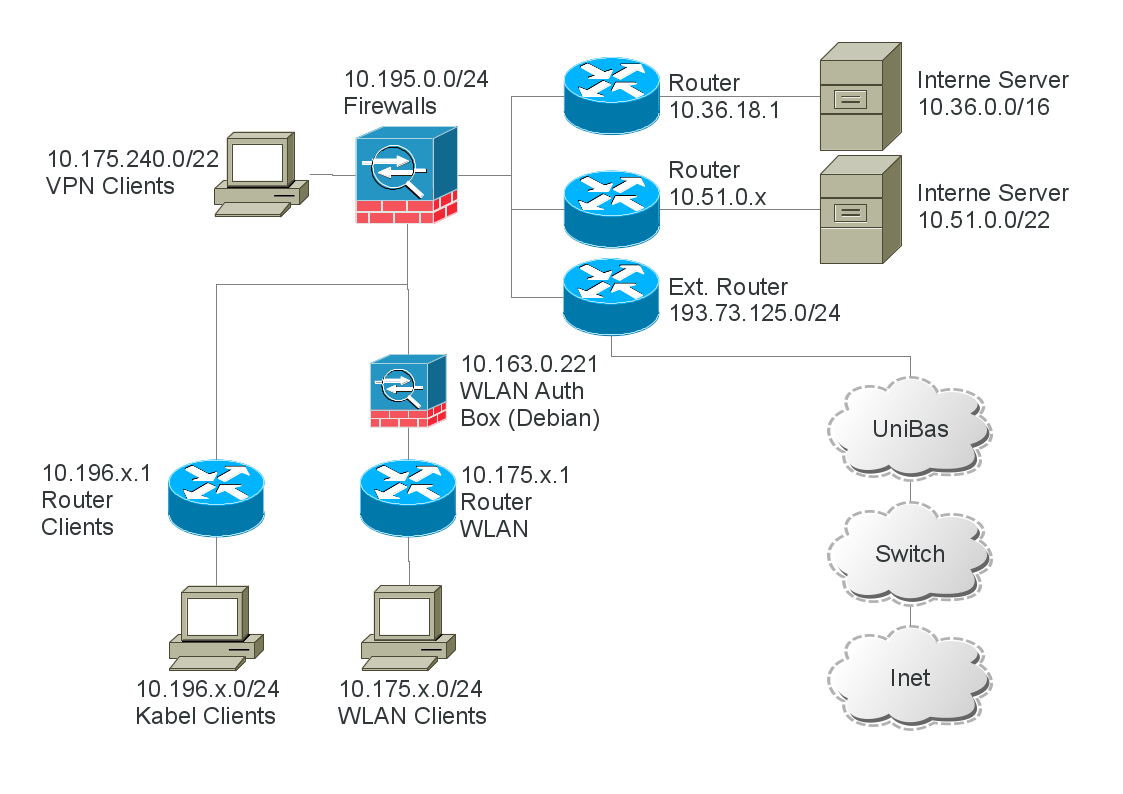
\includegraphics[width=1.0\textwidth]{../aufg5/netzplan.png}
	\caption{Netzwerk FHNW}
	\label{fig:netzplan}
\end{figure}

\subsubsection{Hosts-Tabelle nach den Scans}
Die folgenden Daten wurden aus Metasploit exportiert.
\begin{lstlisting}
msf > hosts -c address,name,os_name -o /tmp/hosts.csv
[*] Wrote hosts to /tmp/hosts.csv
\end{lstlisting}
\begin{longtable}{p{2.5cm}|p{8cm}|l}
	\textbf{address} & \textbf{name} & \textbf{os name}\\
	\hline
	\endfirsthead
	\textbf{address} & \textbf{name} & \textbf{os name}\\
	\hline
	\endhead
	\hline
	\multicolumn{2}{l}{\textit{Fortführung auf nächster Seite\ldots}} \\
	\endfoot
	\endlastfoot
	10.36.19.65 & wi18as33001.adm.ds.fhnw.ch & Unknown\\
	10.36.19.67 & wi18as33003.adm.ds.fhnw.ch & Unknown\\
	10.36.19.69 & wi18as33005.adm.ds.fhnw.ch & Unknown\\
	10.36.19.70 & wi18as33006.adm.ds.fhnw.ch & Unknown\\
	10.36.19.71 & wi18as33007.adm.ds.fhnw.ch & Microsoft Windows\\
	10.36.19.72 & wi18as33008.adm.ds.fhnw.ch & Linux\\
	10.36.19.75 & wi18as33011.adm.ds.fhnw.ch & Unknown\\
	10.36.19.83 & wi18as33019.adm.ds.fhnw.ch & Unknown\\
	10.36.19.84 & wi18as33020.adm.ds.fhnw.ch & Unknown\\
	10.36.19.91 & wi18as33027.adm.ds.fhnw.ch & Unknown\\
	10.36.19.92 & wi18as33028.adm.ds.fhnw.ch & Unknown\\
	10.36.19.99 & wi18as33035.adm.ds.fhnw.ch & Linux\\
	10.36.130.24 & wi18ac34034.adm.ds.fhnw.ch & Unknown\\
	10.36.138.61 & esx11.cs.technik.fhnw.ch & Unknown\\
	10.36.138.62 & esx12.cs.technik.fhnw.ch & Unknown\\
	10.36.138.100 & soleil-int.cs.technik.fhnw.ch & Linux\\
	10.36.138.117 & ci-dotnet.cs.technik.fhnw.ch & Unknown\\
	10.36.138.132 & appris-win.cs.technik.fhnw.ch & Unknown\\
	10.36.138.145 & artichoke-adm.cs.technik.fhnw.ch & Unknown\\
	10.36.139.1 &  & Unknown\\
	10.36.139.27 & vcenter-sgi.cs.technik.fhnw.ch & Unknown\\
	10.36.139.126 & wodss.cs.technik.fhnw.ch & Linux\\
	10.36.139.127 & artichoketest.cs.technik.fhnw.ch & Unknown\\
	10.36.139.128 & sol-idl.cs.technik.fhnw.ch & Linux\\
	10.36.139.129 & tfs10.cs.technik.fhnw.ch & Unknown\\
	10.36.139.130 & ci-stud.cs.technik.fhnw.ch & Linux\\
	10.36.139.132 & rhessi.cs.technik.fhnw.ch & Linux\\
	10.36.139.133 & sensoplus-adm.cs.technik.fhnw.ch & Unknown\\
	10.36.139.134 &  & Linux\\
	10.36.139.135 &  & Linux\\
	10.36.139.140 & iforum.cs.technik.fhnw.ch & Linux\\
	10.36.139.143 & materialdatenbank.cs.technik.fhnw.ch & Unknown\\
	10.36.139.145 & ip-111-pacs-test.cs.technik.fhnw.ch & Linux\\
	10.36.139.147 & ci-android.cs.technik.fhnw.ch & Linux\\
	10.36.139.149 & scavenger.cs.technik.fhnw.ch & Linux\\
	10.36.139.150 & efalg-edu.cs.technik.fhnw.ch & Unknown\\
	10.36.139.152 & woipv.cs.technik.fhnw.ch & Linux\\
	10.36.139.153 & webdog-adm.cs.technik.fhnw.ch & Linux\\
	10.36.139.154 & agilewall-adm.cs.technik.fhnw.ch & Linux\\
	10.36.139.155 &  & Linux\\
	10.51.2.24 &  & Microsoft Windows\\
	10.51.2.25 & mxamu21.adm.ds.fhnw.ch & Unknown\\
	10.51.2.26 & mxamu22.adm.ds.fhnw.ch & Unknown\\
	10.51.2.37 & mxemu24.edu.ds.fhnw.ch & Unknown\\
	10.51.2.38 & mxemu25.edu.ds.fhnw.ch & Unknown\\
	10.51.2.39 & mxemu26.edu.ds.fhnw.ch & Unknown\\
	10.51.2.40 &  & Microsoft Windows\\
	10.51.2.41 &  & Microsoft Windows\\
	10.51.2.64 & mxamu14.adm.ds.fhnw.ch & Unknown\\
	10.51.2.65 & mxamu15.adm.ds.fhnw.ch & Unknown\\
	10.51.2.72 & mxemu14.edu.ds.fhnw.ch & Unknown\\
	10.51.2.73 & mxemu15.edu.ds.fhnw.ch & Unknown\\
	10.51.2.85 &  & Microsoft Windows\\
	10.51.2.150 &  & Microsoft Windows\\
	10.51.2.152 &  & Microsoft Windows\\
	10.51.2.154 &  & Microsoft Windows\\
	10.51.2.155 &  & Microsoft Windows\\
	10.51.2.156 &  & Microsoft Windows\\
	10.51.2.157 &  & Microsoft Windows\\
	10.51.2.158 &  & Microsoft Windows\\
	10.51.2.160 &  & Microsoft Windows\\
	10.51.2.162 &  & Microsoft Windows\\
	10.51.2.164 &  & Microsoft Windows\\
	10.51.2.166 &  & Microsoft Windows\\
	10.51.2.168 &  & Microsoft Windows\\
	10.51.2.172 &  & Microsoft Windows\\
	10.51.2.173 &  & Microsoft Windows\\
	10.51.2.196 &  & Microsoft Windows\\
	10.51.2.204 &  & Microsoft Windows\\
	10.51.2.207 &  & Microsoft Windows\\
	10.51.3.32 & psemu11.edu.ds.fhnw.ch & Unknown\\
	10.51.3.33 & psemu12.edu.ds.fhnw.ch & Unknown\\
	10.51.3.34 & psemu15.edu.ds.fhnw.ch & Unknown\\
	10.51.3.35 & psemu16.edu.ds.fhnw.ch & Unknown\\
	10.51.3.37 & psemu18.edu.ds.fhnw.ch & Unknown\\
	10.51.3.41 & psemu19.edu.ds.fhnw.ch & Unknown\\
	10.51.3.42 & psemu21.edu.ds.fhnw.ch & Unknown\\
	10.51.3.46 & asamu25.adm.ds.fhnw.ch & Unknown\\
	10.51.3.51 & asara115.adm.ds.fhnw.ch & Unknown\\
	10.51.3.52 & asara116.adm.ds.fhnw.ch & Unknown\\
	10.51.3.73 & asemu13.edu.ds.fhnw.ch & Unknown\\
	10.51.3.74 & osamu25.adm.ds.fhnw.ch & Unknown\\
	10.51.3.76 & network.services.fhnw.ch & Unknown\\
	10.51.3.78 & asamu46.adm.ds.fhnw.ch & Unknown\\
	10.51.3.91 & psera112.edu.ds.fhnw.ch & Unknown\\
	10.51.3.99 & psera111.edu.ds.fhnw.ch & Unknown\\
	10.51.3.129 & asara133.adm.ds.fhnw.ch & Unknown\\
	10.51.3.130 & osara111.adm.ds.fhnw.ch & Unknown\\
	10.51.3.140 & webmail.fhnw.ch & Unknown\\
	10.51.3.144 & casarray.adm.ds.fhnw.ch & Unknown\\
	10.51.3.146 & legacy.fhnw.ch & Unknown\\
	10.51.4.16 & acs30u101.net.fhnw.ch & Unknown\\
	10.51.4.17 & acs30u102.net.fhnw.ch & Unknown\\
	10.163.0.221 & mpp30u101-dok.net.fhnw.ch & Linux\\
	10.196.136.1 &  & Unknown\\
	10.196.136.21 & fwg114p.edu.ds.fhnw.ch & Unknown\\
	10.196.136.118 &  & Unknown\\
	10.196.136.120 &  & Unknown\\
	147.86.3.40 & wsnra113.fhnw.ch & Linux\\
	147.86.3.42 & asemu17.ict.fhnw.ch & Unknown\\
	147.86.3.43 & tools.fhnw.ch & Linux\\
	147.86.3.44 & sapportal.fhnw.ch & Linux\\
	147.86.3.45 & sapportaltest.fhnw.ch & Linux\\
	147.86.3.47 & aai-logon.test.fhnw.ch & Linux\\
	147.86.3.48 & es.fhnw.ch & Linux\\
	147.86.3.51 & tools4.fhnw.ch & Linux\\
	147.86.3.52 & wsnmu27-sec4.fhnw.ch & Unknown\\
	147.86.3.55 & aai-logon.fhnw.ch & Linux\\
	147.86.3.56 & asnra113.fhnw.ch & Unknown\\
	147.86.3.57 & asnra113-sec1.fhnw.ch & Unknown\\
	147.86.3.58 & asnra113-sec2.fhnw.ch & Unknown\\
	147.86.3.59 & asnra113-sec3.fhnw.ch & Unknown\\
	147.86.3.66 & web.fhnw.ch & Linux\\
	147.86.3.67 & webz.fhnw.ch & Linux\\
	147.86.3.68 & web.asa.fhnw.ch & Linux\\
	147.86.3.69 & pmst.fhnw.ch & Linux\\
	147.86.3.76 & webtransfer.fhnw.ch & Linux\\
	147.86.3.88 & mail.fhnw.ch & Unknown\\
	147.86.3.89 & legacy.fhnw.ch & Unknown\\
	147.86.3.100 & moodle.test.fhnw.ch & Unknown\\
	147.86.3.101 & moodle3.test.fhnw.ch & Unknown\\
	147.86.3.160 & wsnmu25.fhnw.ch & Unknown\\
	147.86.3.161 & wsnmu25-sec1.fhnw.ch & Unknown\\
	147.86.3.162 & wsnmu25-sec2.fhnw.ch & Unknown\\
	147.86.3.163 & wsnmu25-sec3.fhnw.ch & Unknown\\
	147.86.3.164 & wsnmu32.fhnw.ch & Linux\\
	147.86.3.165 & wsnmu32-sec1.fhnw.ch & Linux\\
	147.86.3.166 & wsnmu32-sec2.fhnw.ch & Linux\\
	147.86.3.167 & wsnmu32-sec3.fhnw.ch & Linux\\
	147.86.3.168 & wsnmu32-sec4.fhnw.ch & Unknown\\
	147.86.3.169 & wsnmu32-sec5.fhnw.ch & Linux\\
	147.86.3.170 & wsnmu31.fhnw.ch & Unknown\\
	147.86.3.171 & wsnmu31-sec1.fhnw.ch & Unknown\\
	147.86.3.172 & wsnmu31-sec2.fhnw.ch & Unknown\\
	147.86.3.173 & wsnmu31-sec3.fhnw.ch & Unknown\\
	147.86.3.174 & wsnmu31-sec4.fhnw.ch & Unknown\\
	147.86.3.175 & wsnmu31-sec5.fhnw.ch & Unknown\\
	147.86.3.176 & wsnmu33.fhnw.ch & Unknown\\
	147.86.3.177 & wsnmu33-sec1.fhnw.ch & Unknown\\
	147.86.3.178 & wsnmu33-sec2.fhnw.ch & Unknown\\
	147.86.3.179 & wsnmu33-sec3.fhnw.ch & Unknown\\
	147.86.3.180 & wsnmu33-sec4.fhnw.ch & Unknown\\
	147.86.3.182 & wsnmu14.fhnw.ch & Linux\\
	147.86.3.183 & wsnmu37.fhnw.ch & Unknown\\
	147.86.3.184 & wsnmu37-sec1.fhnw.ch & Unknown\\
	147.86.3.185 & wsnmu37-sec2.fhnw.ch & Unknown\\
	147.86.3.186 & wsnmu37-sec3.fhnw.ch & Unknown\\
	147.86.3.187 & wsnmu37-sec4.fhnw.ch & Unknown\\
	147.86.3.188 & wsnmu37-sec5.fhnw.ch & Unknown\\
	147.86.3.189 & wsnmu37-sec6.fhnw.ch & Unknown\\
	147.86.3.190 & wsnmu37-sec7.fhnw.ch & Unknown\\
	147.86.3.201 & wsnmu33-sec11.fhnw.ch & Unknown\\
	147.86.3.202 & wsnmu33-sec12.fhnw.ch & Unknown\\
	147.86.3.203 & wsnmu33-sec13.fhnw.ch & Unknown\\
	147.86.3.204 & wsnmu33-sec14.fhnw.ch & Unknown\\
	147.86.3.205 & wsnmu33-sec15.fhnw.ch & Unknown\\
	147.86.3.206 & wsnmu33-sec16.fhnw.ch & Unknown\\
	147.86.3.207 & wsnmu33-sec17.fhnw.ch & Unknown\\
	147.86.3.208 & wsnmu33-sec18.fhnw.ch & Unknown\\
	147.86.3.209 & wsnmu33-sec19.fhnw.ch & Unknown\\
	147.86.3.210 & wsnra111.fhnw.ch & Unknown\\
	147.86.3.211 & wsnra111-sec1.fhnw.ch & Unknown\\
	147.86.3.212 & wsnra111-sec2.fhnw.ch & Unknown\\
	147.86.3.213 & wsnra111-sec3.fhnw.ch & Unknown\\
	147.86.3.214 & wsnra111-sec4.fhnw.ch & Unknown\\
	147.86.3.215 & wsnra111-sec5.fhnw.ch & Unknown\\
	147.86.3.239 & vpn1.fhnw.ch & Unknown\\
	147.86.3.240 & vpn2.fhnw.ch & Unknown\\
	147.86.7.16 & ba19ns10001.adm.ds.fhnw.ch & Unknown\\
	147.86.7.17 & webcorp2.fhnw.ch & Unknown\\
	147.86.7.18 & evasys.ph.fhnw.ch & Microsoft Windows\\
	147.86.7.20 & baselonthemove.ivgi.habg.fhnw.ch & Microsoft Windows\\
	147.86.7.21 & genius.wirtschaft.fhnw.ch & Unknown\\
	147.86.7.22 & promere.ivgi.habg.fhnw.ch & Microsoft Windows\\
	147.86.7.23 & ol19ns11003.adm.ds.fhnw.ch & Microsoft Windows\\
	147.86.7.24 & aa16as00222.adm.ds.fhnw.ch & Unknown\\
	147.86.7.25 & www.mab-bs.ch & Linux\\
	147.86.7.26 & rechtsgrundlagen.wirtschaft.fhnw.ch & Unknown\\
	147.86.7.28 & collaboration.ivgi.habg.fhnw.ch & Unknown\\
	147.86.7.29 & elo.wirtschaft.fhnw.ch & Unknown\\
	147.86.7.30 & planer.mab-bs.ch & Linux\\
	147.86.7.33 & so16ns00001.fhnw.ch & Linux\\
	147.86.7.34 & www.rimab.ch & Linux\\
	147.86.7.36 & ba23ns00009.fhnw.ch & Linux\\
	147.86.8.16 & loki.cs.technik.fhnw.ch & Unknown\\
	147.86.8.22 & ftm1.cs.technik.fhnw.ch & Unknown\\
	147.86.8.26 & janus.imvs.technik.fhnw.ch & Linux\\
	147.86.8.27 & helios.cs.technik.fhnw.ch & Unknown\\
	147.86.8.30 & inf7550a.cs.technik.fhnw.ch & Linux\\
	147.86.8.39 & galaxy3.cs.technik.fhnw.ch & Linux\\
	147.86.8.40 & galaxy4.cs.technik.fhnw.ch & Linux\\
	147.86.8.41 & galaxy5.cs.technik.fhnw.ch & Linux\\
	147.86.8.74 & i4dsweb.cs.technik.fhnw.ch & Linux\\
	147.86.8.75 & datalogger.cs.technik.fhnw.ch & Linux\\
	147.86.8.76 & feinstaub.cs.technik.fhnw.ch & Linux\\
	147.86.8.80 & soleil80.cs.technik.fhnw.ch & Unknown\\
	147.86.8.81 & dbau.cs.technik.fhnw.ch & Linux\\
	147.86.8.82 & hespe.cs.technik.fhnw.ch & Linux\\
	147.86.8.83 & desdm.cs.technik.fhnw.ch & Linux\\
	147.86.8.84 & stix.cs.technik.fhnw.ch & Linux\\
	147.86.8.97 & crm-blueconomics.cs.technik.fhnw.ch & Unknown\\
	147.86.8.98 & iCompetence-Workspace.cs.technik.fhnw.ch & Linux\\
	147.86.8.99 & iCompetence-Webdesign.cs.technik.fhnw.ch & Linux\\
	147.86.8.101 & project.cs.technik.fhnw.ch & Linux\\
	147.86.8.102 & helio.cs.technik.fhnw.ch & Linux\\
	147.86.8.104 & plone3.cs.technik.fhnw.ch & Linux\\
	147.86.8.105 & helio2.cs.technik.fhnw.ch & Linux\\
	147.86.8.106 & hedc.cs.technik.fhnw.ch & Linux\\
	147.86.8.108 & bbbgrades.cs.technik.fhnw.ch & Linux\\
	147.86.8.111 & focalpoint.cs.technik.fhnw.ch & Linux\\
	147.86.8.112 & blueconomics.cs.technik.fhnw.ch & Linux\\
	147.86.8.113 & jobcrawler.cs.technik.fhnw.ch & Unknown\\
	147.86.8.114 & jobcrawler2.cs.technik.fhnw.ch & Unknown\\
	147.86.8.158 & aps123.cs.technik.fhnw.ch & Linux\\
	147.86.8.159 & aps2.cs.technik.fhnw.ch & Linux\\
	147.86.8.160 & aps3.cs.technik.fhnw.ch & Linux\\
	147.86.8.171 & helio-dev.cs.technik.fhnw.ch & Linux\\
	147.86.8.185 & web.cs.technik.fhnw.ch & Unknown\\
	147.86.8.192 & streaming.cs.technik.fhnw.ch & Unknown\\
	147.86.8.194 & livingvindonissa.cs.technik.fhnw.ch & Linux\\
	147.86.8.195 & plone.cs.technik.fhnw.ch & Linux\\
	147.86.8.196 & webapache.cs.technik.fhnw.ch & Linux\\
	147.86.8.197 & lis.imvs.technik.fhnw.ch & Linux\\
	147.86.8.200 & sjf.cs.technik.fhnw.ch & Linux\\
	147.86.8.203 & systemservices.cs.technik.fhnw.ch & Unknown\\
	147.86.8.209 & webdb.cs.technik.fhnw.ch & Linux\\
	147.86.8.210 & codechecker.cs.technik.fhnw.ch & Linux\\
	147.86.8.213 & dk.cs.technik.fhnw.ch & Linux\\
	147.86.8.214 & sdent.cs.technik.fhnw.ch & Linux\\
	147.86.8.216 & vm167.cs.technik.fhnw.ch & Linux\\
\end{longtable}

\end{document}